\documentclass[a4paper,titlepage,12pt]{article}
\usepackage[utf8]{inputenc} %Make sure all UTF8 characters work in the document
\usepackage{color}
\usepackage{graphicx}
\usepackage{titling}
\usepackage[titletoc,title]{appendix}
\usepackage{tabularx}
\usepackage{longtable}
\usepackage[yyyymmdd]{datetime}
\usepackage[figurename=Figur]{caption}
\usepackage{pbox}
\usepackage{booktabs}
\usepackage[parfill]{parskip}
%\usepackage[compact]{titlesec}

%Set page size
\usepackage{geometry}
\geometry{margin=3cm}

\renewcommand{\dateseparator}{-}
\renewcommand{\contentsname}{Innehållsförteckning}
\renewcommand{\appendixname}{Bilaga}

%%%%%%%%%%%%%%%%%%%%%%%%%%%%%%%
% Header and footer
%%%%%%%%%%%%%%%%%%%%%%%%%%%%%%%
\usepackage{fancyhdr}
\pagestyle{fancy}

\lhead{
\includegraphics[width=0.15\linewidth]{../images/logo_full.png}}
\chead{Projektplan för sexbent robot}
\rhead{\today}
\setlength\headheight{26pt} 

\lfoot{TSEA29 --- KMM \\ LIPS Projektplan}
\rfoot{Grupp 9 \\ LiTHe Hex}

\pretitle{%
	\begin{center}
		\LARGE
		
\includegraphics[width=6cm]{../images/logo_full.png}\\[\bigskipamount]
}

\posttitle{\end{center}}

\newcounter{milNr}
\setcounter{milNr}{0}
\newcommand{\nextMilNr}{\stepcounter{milNr}\arabic{milNr}}

\newcounter{bpNr}
\setcounter{bpNr}{0}
\newcommand{\nextBPNr}{\stepcounter{bpNr}\arabic{bpNr}}

\newcounter{aktNr}
\setcounter{aktNr}{0}
\newcommand{\nextAktNr}{\stepcounter{aktNr}\arabic{aktNr}}

\begin{document}
	\title{\LARGE
		\textbf{Projektplan för sexbent robot} \\
		\vspace*{0.5\baselineskip}
		\large
		Redaktör Malcolm Vigren \\
		Grupp 9 \\
		\small
		\vspace*{0.5\baselineskip}
		Version 0.3}

	\date{\today}

		\maketitle
	
	\newpage
	
	\begin{center}

		%%%%%%%%%%%%%%%%%%%%%%%%%%%%%%%%%%%%%%%%%%%%%%%%%%%%%%%%%%%%%%%%%%%%%%%%%%%%%%%%%
		%						Medlemmar
		%%%%%%%%%%%%%%%%%%%%%%%%%%%%%%%%%%%%%%%%%%%%%%%%%%%%%%%%%%%%%%%%%%%%%%%%%%%%%%%%%

		\section*{Projektidentitet}
		Grupp 9, Ht 2016, LiTHe Hex

		Linköpings Tekniska Högskola, ISY

		\renewcommand*{\arraystretch}{1.4}
		\begin{longtable}[c]{ l l l }
			\textbf{Namn} & \textbf{Ansvar} & \textbf{E-post} \\ \midrule
			Emil Segerbäck & & emise935@student.liu.se \\ \midrule
			Frans Skarman & Dokumentansvarig & frask812@student.liu.se \\ \midrule
			Hannes Tuhkala & & hantu447@student.liu.se \\ \midrule
			Malcolm Vigren & Projektledare & malvi108@student.liu.se \\ \midrule
			Noak Ringman &  & noari093@student.liu.se \\ \midrule
			Olav Övrebö &  & olaov121@student.liu.se \\ \midrule
			Robin Sliwa & & robsl733@student.liu.se \\
		\end{longtable}

		\centering
		\textbf{Kursansvarig}: Tomas Svensson Rum 3B:528 013--28 13 68 tomas.svensson@liu.se

		\newpage
		\tableofcontents
		\newpage


		%%%%%%%%%%%%%%%%%%%%%%%%%%%%%%%%%%%%%%%%%%%%%%%%%%%%%%%%%%%%%%%%%%%%%%%%%%%%%%%%%
		%						Historik
		%%%%%%%%%%%%%%%%%%%%%%%%%%%%%%%%%%%%%%%%%%%%%%%%%%%%%%%%%%%%%%%%%%%%%%%%%%%%%%%%%

		\section*{Dokumenthistorik}
		\renewcommand*{\arraystretch}{1.4}
        \begin{longtable}[c]{ l l l >{\raggedright}p{3cm} l }
			\textbf{Version} & \textbf{Datum} & \textbf{Utförda förändringar} 
			& \textbf{Utförda av} & \textbf{Granskad} \\ \midrule

			0.1 & 2016--09--20 & Första utkastet & Projektgruppen & Projektgruppen\\
			0.2 & 2016--09--27 & Andra utkastet & MV, RS & TS \\
			0.3 & 2016--09--28 & Tredje utkastet & MV, RS, ES, HT, NR, FS & \\
		\end{longtable}
	\end{center}

	\newpage

	\section{Beställare}
	Beställare är Tomas Svensson, lektor vid Linköpings tekiska högskola. \\
  Kontaktdata: Rum 3B:528 013–28 13 68 tomas.svensson@liu.se

	%%%%%%%%%%%%%%%%%%%%%%%%%%%%%%%%%%%%%%%%%%%%%%%%%%%%%%%%%%%%%%%%%%%%%%%%%%%%%%%%%
	%						Översikt
	%%%%%%%%%%%%%%%%%%%%%%%%%%%%%%%%%%%%%%%%%%%%%%%%%%%%%%%%%%%%%%%%%%%%%%%%%%%%%%%%%

	\section{Översiktlig beskrivning av projektet}
	Projektet är en del av kursen \textit{Konstruktion med mikrodatorer} där en
  projektgrupp ska konstruera en sexbent robot. 

	\subsection{Syfte och mål}
	Syftet och målet med projektet är att utveckla en sexbent robot som själv
	kan navigera sig ut ur en labyrint. I labyrinten bör roboten även kunna ta
	sig över hinder för att komma vidare.

	
	\subsection{Leveranser}
	De dokument som ska levereras till kunden är: projektplan, tidplan,
	systemskiss, designspecifikation, teknisk dokumentation och
	användarhandledning. Slutleveransen består av en presentation av projektet,
	demonstration av roboten i autonomnt och manuellt läge i form av en tävling,
	samt överlämning av kod, hårdvara och dokumentation.

	\begin{longtable}[l]{l l}
		\textbf{Leverans} & \textbf{Leveransdatum} \\ \midrule
		
		Projektplan & 2016--09--29 \\ \midrule

		Tidplan & 2016--09--29  \\ \midrule
		
		Systemskiss & 2016--09--29 \\ \midrule

		Designspecifikation & 2016--11--04 \\ \midrule

		Tidrapporter & 31/10, 7/11, 14/11, 21/11, 28/11, 5/12, 12/12, 19/12
                   -- 2016		\\ \midrule

		Teknisk dokumentation & 2016--12--17 \\ \midrule

		Användarhandledning & 2016--12--17 \\ \midrule

        Slutleverans & Vecka 51, 2016 \\ \midrule

		Efterstudie & 2016--12--21  \\ \midrule
	\end{longtable}
	
	
	\subsection{Begränsningar}
	Roboten behöver inte klara mer avancerade former på labyrinten än de som
	beskrivs i Ban- och regelspecifikationen.
	
	
	\section{Fasplan}
    Projektet har två huvudfaser efter inledningsfasen - "Under"-fasen samt
    "Efter"-fasen. Under-fasen är den fas då själva konstruktionen designas, 
    implementeras samt dokumenteras, och Efter-fasen innehåller det arbetet som
    ska göra efter att konstruktionen är klar.
	
	\subsection{Under projektet}
	Under projektet ska en designspecifikation skrivas med detaljerad
	information om hur roboten ska implementeras. Efter att
	designspecifikationen är klar påbörjas implementationen av systemet. Vid
    denna tidpunkt ska simuleringar konstrueras för att underlätta testning av
    delar av systemet innan hela systemet har implementerats.
	Enhetstester ska konstrueras i takt med att testbara delar av systemet har
	implementerats. Teknisk dokumentation för varje delsystem ska skrivas
	i takt med att implementationsbeslut utförs.

	Hela gruppen ska ha möten minst en gång per vecka för att presentera
	varandras arbete sedan förra mötet, och för att kontrollera att projektet
	följer planen. Dessa möten blir också tillfällen att diskutera problem som
	uppstår med hela gruppen.

	Om ett visst krav i kravspecifikationen inte kan implementeras ska ett möte
	med beställaren anordnas för omförhandling av kravet i fråga.
	
	\subsection{Efter projektet}
	Projektet avslutas med slutleverans efter att alla krav i
	kravspecifikationen är uppfyllda. Efter leveransen görs en efterstudie.
	
	
	\section{Organisationsplan för hela projektet}
	%I detta avsnitt beskrivs hur projektet ska organiseras.
	Projektrollerna som ingår i detta projekt är: beställare/kund, handlerare,
	projekt-ledare och projektmedlemmar. Alla projektmedlemmar har kontakt med
	hand-ledaren, men det är projektledaren som sköter den huvudsakliga
	kontakten med beställaren, se figur~\ref{fig:organization}.

	\begin{figure}[h!]
		\begin{center}
		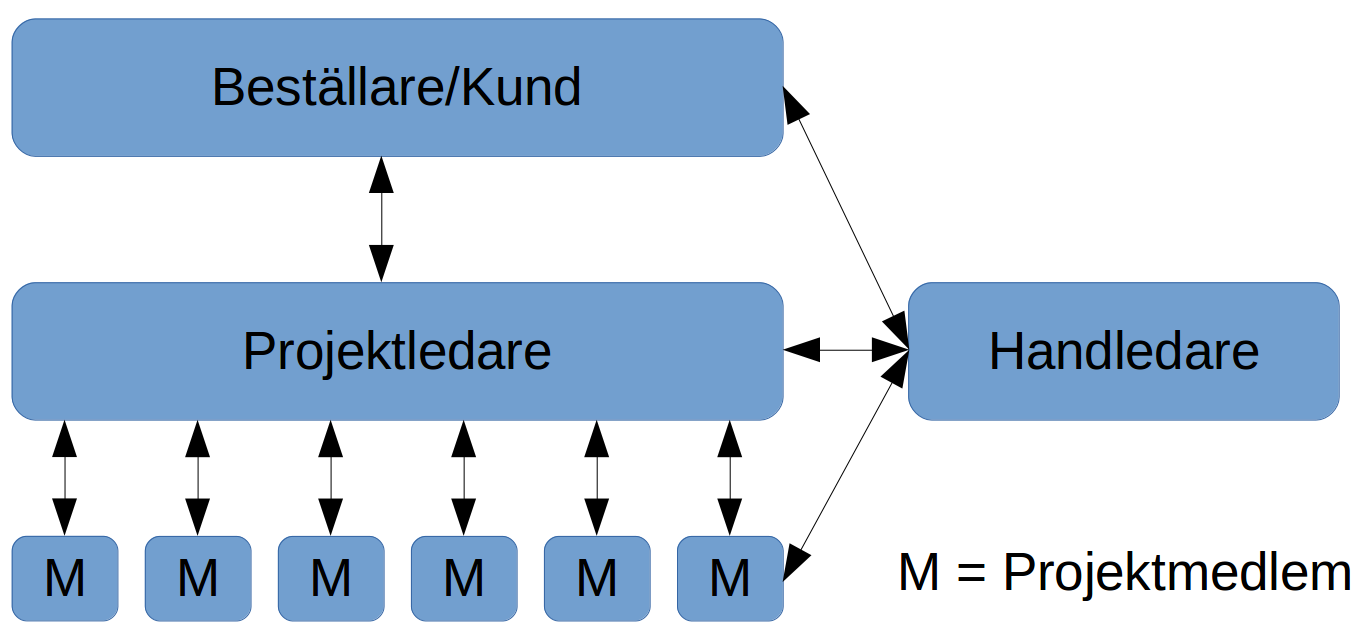
\includegraphics[width=0.8\linewidth]{images/projectroles.png}
		\caption{Projektets organisation\label{fig:organization}}
		\end{center}
	\end{figure}
	 
	\subsection{Villkor för samarbetet inom projektgruppen}
    Gruppen har kommit överens om villkor för samarbetet, och formulerat det i
    ett internt gruppkontrakt för samarbete.
	
	\subsection{Definition av arbetsinnehåll och ansvar}
	Beställarens huvudsakliga uppgifter är att fatta beslut
	om fortsättning av projektet vid beslutspunkter, godkänna
	ändringar under projektets gång, läsa statusrapporter samt godkännande av
	projektets avslut. Arbetsuppgifterna för projektledaren är, utöver
	arbetsuppgifterna för resten av projektmedlemmarna, att fördela
	arbets-uppgifter, planera och leda projektarbetet, se till att projektets mål
	nås samt \\ motivera projektmedlemmarna.

	Kommunikationen mellan projektmedlemmar kommer att ske genom möten, en
	gemensam kalender samt en gruppchatt.
	
	För information om hur arbetet på delsystemen ska fördelas, se Bilaga
	A - Tidplan.
	
	\section{Dokumentplan}
	GitHub och Git används för versionshantering av
	dokumenten, som skrivs i LaTeX. Alla projektmedlemmar har tillgång till
	samtliga dokument. All dokumentation, förutom kommentarer och doc-strängar
	i kod, är skriven på svenska.

	Stora ändringar ger inkrementering av heltalssiffran i versionsnumrena,
	medan små ändringar ger inkrementation av decimalsiffran.
	
	\begin{longtable}[l]{ p{3cm} p{3.2cm} >{\raggedright}p{5cm} p{2.2cm} l }
		\textbf{Dokument} & \textbf{Ansvarig/ godkänns av} & \textbf{Syfte} & \textbf{Färdigdatum} \\ \midrule
		
		Kravspeci-fikation & Dokumentansvarig /Beställare & Definierar alla krav på systemet & 2016--09--13 \\ \midrule

		Projektplan & Projektledare /Beställare & Beskrivning av hur projektet ska genomföras & 2016--09--29 \\ \midrule

		Tidplan & Projektledare /Beställare & Planering för hur arbetstid ska fördelas. & 2016--09--29  \\ \midrule
		
		Systemskiss & Dokumentansvarig /Beställare & Grov skiss och idéer för implementation av systemet & 2016--09--29 \\ \midrule

        Gruppkontrakt & Projektledare /Projektledare & Interna villkor för samarbete inom
        gruppen & 2016--09--23 \\ \midrule

		Designspeci-fikation & Dokumentansvarig /Handledare & Detaljerad beskrivning av implementationen av systemet. & 2016--11--04 \\ \midrule

		Tidrapporter & Projektledare /Beställare & Rapportering av använd arbetstid & Veckovis		\\ \midrule

		Statusrapporter & Projektledare /Beställare & Rapportering av nuvarande framsteg & Veckovis \\ \midrule

		Teknisk dokumentation & Dokumentansvarig /Beställare & Teknisk beskriving av
		implementationen av den färdiga produkten. & 2016--12--17 \\ \midrule

		Användar-handledning & Dokumentansvarig /Beställare & Manual för användning av produkten & 2016--12--17 \\ \midrule

		Efterstudie & Dokumentansvarig /- & Utvärdering av projektet & 2016--12--22  \\ \midrule
	\end{longtable}
	
	
	\section{Utvecklingsmetodik}
	För programmering av AVR-processorerna i sensor- och motorikenheten ska C
	användas. För programmering av centralenheten ska Python användas, då det
	är ett högnivå-språk med bra stöd i Raspberry Pi. GUI-systemet ska
	programmeras i det funktionella språket Elm. All kod versionshanteras med Git.
	
	\section{Utbildningsplan}

	De gruppmedlemmar som arbetar på ett visst delsystem bör vara fullt
	utbildade i alla tekniska detaljer som ingår i implementationen av det
	delsystemet. Gruppmedlemmar som arbetar på andra system behöver inte lika
	stor insikt i de tekniska \\ detaljerna, men bör
	informera sig om gränssnitten mellan sin enhet och andra delsystem, samt väldigt 
	grundläggande information om hur enheterna är uppbyggda och om deras syften.

	Varje delgrupp är ansvarig i att utbilda sig inom de kunskaper som krävs
	för utveckling av sina respekive delsystem. Den utsatta tiden för
	aktiviteterna innefattar även tiden det tar att utbilda sig. 

	\section{Rapporteringsplan}
	Tids- och statusrapporter ska skrivas och skickas in följande datum innan kl 16:00: 
    2016--10--31, 2016--11--07, 2016--11--14, 2016--11--21, 2016--11--28, 2016--12--05, 
    2016--12--12 och 2016--12--19. Den utvalda sekreteraren för det mötet skriver tids-
    och statusrapport som granskas och skickas in av projektledaren. 
	
	\section{Mötesplan}
	Minst en gång per vecka ska ett möte hållas, där alla gruppmedlemmar
	redovisar för vad de har gjort, vilka problem de har löst, samt hur de
	tänker fortsätta sitt arbete. Mötena ska även användas för diskussion av
	problem gällande de olika delsystemen eller hela systemet. Dessa möten väntas 
	ta ungefär 1 timme, och vid varje möte ska en sekreterare utses, som åläggs skriva 
	en statusrapport utifrån det som tagits upp på mötet. Mötena ska ske i början av
	varje vecka, oftast första lediga tid i schemat under måndagen.
	
	\section{Resursplan}
  
	\subsection{Personer}
	Alla 7 projektmedlemmar förväntas arbeta ungefär lika mycket under alla
	projektfaser. Projektgruppen har tillgång till en handlerare 2 timmar per vecka. 
	
	\subsection{Material}
    I nuläget är det känt att följande material behövs:
	\begin{itemize}
			\item Chassi för hexapod-robot inklusive servon
			\item 2 AVR-processorer
			\item 1 Raspberry Pi-enkortsdator (3:e generationen)
			\item Avståndssensorer
            \item 1 Gyro
            \item Kretskort
            \item Diverse kablar och elektronikkomponenter
	\end{itemize}
	
	
	\subsection{Lokaler}
	Muxen kommer användas för kodning och testning med robot. Grupprum kommer
	användas för kodning, design och möten.
	
	
	\subsection{Ekonomi}
	Efter godkänd projektplan får maximalt 1120 arbetstimmar ha använts på projektet.
	
	
	\section{Milstolpar och beslutspunkter}
	Milstolparna består av viktiga delmoment och avslutade projektfaser som
	spelar kritisk roll. 
	
	\subsection{Milstolpar}
	\begin{longtable}[c]{ c l c}
		\textbf{Nr} & \textbf{Beskrivning} & \textbf{Datum} \\ \midrule
		\nextMilNr{} & Designspecifikation är klar & 2016--11--04 \\ \midrule
		\nextMilNr{} & Roboten kan kontrollera servona med inverterad kinematik
        & 2016--11--26 \\ \midrule
		\nextMilNr{} & Det går att styra roboten från gränssnittet &
        2016--12--02 \\ \midrule
		\nextMilNr{} & Roboten kan fatta beslut med hjälp av sensordata &
        2016--12--09 \\ \midrule
		\nextMilNr{} & Roboten kan navigera sig igenom en bana enligt
        specifikationen & 2016--12--12 \\ \midrule
		\nextMilNr{} & Teknisk dokumentation är klar & 2016--12--14 \\ \midrule
	\end{longtable}
	
	
	\subsection{Beslutspunkter}
	\renewcommand*{\arraystretch}{1.4}
    \begin{longtable}[c]{ c p{0.8\textwidth} c}
		\textbf{Nr} & \textbf{Beskrivning} & \textbf{Datum} \\ \midrule
		\nextBPNr{} & Godkännande av projektdirektiv, beslut att starta förstudie & 2016--09--02 \\ \midrule
		\nextBPNr{} & Godkännande av kravspecifikation, beslut att starta förberedelsefasen & 2016--09--13 \\ \midrule
		\nextBPNr{} & Godkännande av projektplanering, beslut att starta utförandefasen & 2016--09--29 \\ \midrule
		\nextBPNr{} & Godkännande av designspecifikation, beslut att fortsätta
		utförandefasen & 2016--11--04 \\ \midrule
		\nextBPNr{} & Godkännande av produktens funktionalitet, beslut att
        leverera & Vecka 50, 2016 \\ \midrule
		\nextBPNr{} & Godkännande av leverans, beslut att upplösa projektgruppen & -- \\ \midrule
	\end{longtable}
	
	
	\section{Aktiviteter}
	\renewcommand*{\arraystretch}{1.4}
	\begin{longtable}[c]{ c p{4cm} p{6cm} p{2cm} p{2cm}}
		\textbf{Nr} & \textbf{Aktivitet} & \textbf{Beskrivning} & \textbf{Beroende av nr} & \textbf{Beräknad tid (tim)} \\ \midrule
		\nextAktNr{} & Inverterad Kinematik & Uträkning av vinklar för servon utifrån slutposition &  & 30 \\ \midrule
		\nextAktNr{} & Servokontroll & Kunna kontrollera servon &  & 16 \\ \midrule
		\nextAktNr{} & Gångstil & Hur roboten går åt olika håll & 1 & 50 \\ \midrule
		\nextAktNr{} & Kommunikation centralenhet & Motorikenheten ska kommunicera med centralenheten &  & 10 \\ \midrule
		\nextAktNr{} & Golvhöjdsdetektion & Detektering av höjdskillnader i banan & 2 & 20 \\ \midrule
		\nextAktNr{} & Stötdetektion av hinder & Upptäcka stöt med hinder & 2 & 15 \\ \midrule
		\nextAktNr{} & Hindergång & Ta sig över hinder på banan & 1,3 & 40 \\ \midrule
		\nextAktNr{} & Enhetstestning & Enhetstestning av motorikenhetens komponenter & & 5 \\ \midrule
		\nextAktNr{} & Kommunikation med motorikenhet & Centralenhetens kommunikation med motorikenheten &  & 10 \\ \midrule
		\nextAktNr{} & Detektera återvändsgränder & Detektera återvändsgränder
                                                m.h.a. sensordata &  & 14 \\ \midrule
		\nextAktNr{} & Kommunikation med sensorenhet & Centralenhetens kommunikation
                                                   med sensorenheten &  & 10 \\ \midrule
		\nextAktNr{} & Kommunikation med GUI & Centralenhetens kommunikation med GUI &  & 10 \\ \midrule
		\nextAktNr{} & Följa korridor & Kunna följa en korridor m.h.a. sensordata &  & 20 \\ \midrule
		\nextAktNr{} & Hinderdetektion & Detektera hinder m.h.a. sensordata &  & 22 \\ \midrule
		\nextAktNr{} & Hinderhantering & Gå över hindret efter detektion &  & 22 \\ \midrule
		\nextAktNr{} & Beslutsfattning & Fatta beslut m.h.a. sensordata & 10,13,14,15 & 24 \\ \midrule
		\nextAktNr{} & GUI kommandotolkning & Tolka de kommandon som kommer in från GUI & 12 & 12 \\ \midrule
		\nextAktNr{} & Telemetri & Skicka data till de olika enheterna och GUI & 12 & 12 \\ \midrule
		\nextAktNr{} & Enhetstestning & Enhetstestning av centralenhetens komponenter& & 5 \\ \midrule
		\nextAktNr{} & GUI för manuell styrning & Styra roboten manuellt m.h.a. GUI & 21,22 & 12 \\ \midrule
		\nextAktNr{} & Webbserver & Fungerande webbserver på centralenheten &  & 18 \\ \midrule
		\nextAktNr{} & Kommunikation med webbserver & Frontend kommunikation med webbservern &  & 10 \\ \midrule
		\nextAktNr{} & Joystick-kontroll & Kontroll av robot från GUI m.h.a. en joystick & 20,21,22 & 18 \\ \midrule
		\nextAktNr{} & Visning av debuglog & Visning av data från centralenheten & 21,22 & 10 \\ \midrule
		\nextAktNr{} & Enhetstestning & Enhetstestning av GUI & & 5 \\ \midrule
		\nextAktNr{} & Läsning av avståndssensorer & Läsa av data från avståndssensorer & 33 & 10 \\ \midrule
		\nextAktNr{} & Kommunikation med centralenhet & Sensorenhetens kommunikation
                                                            med centralenheten& 36 & 10 \\ \midrule
		\nextAktNr{} & Läsning av gyro & Läsa av data från gyro & & 10 \\ \midrule
		\nextAktNr{} & Läsning av LIDAR & Läsa av data från LIDAR & & 10 \\ \midrule
		\nextAktNr{} & Brusreduktion av gyro & Brusreduktion av den inlästa gyrodatan & 28 & 16 \\ \midrule
		\nextAktNr{} & Brusreduktion av avståndssensor & Brusreduktion av den
                                                     inlästa avståndsdatan & 26 & 16 \\ \midrule
		\nextAktNr{} & Vinkeluträkning av gyro & Uträkning av vinkel från den
                                             brusreducerade gyrodatan & 28 & 12 \\ \midrule
		\nextAktNr{} & Multiplexning A/D-omvandlare & Multiplexning av A/D omvandlare & & 14 \\ \midrule
		\nextAktNr{} & Enhetskonvertering & Konvertera sensordata till vettiga enheter &  & 10 \\ \midrule
		\nextAktNr{} & Enhetstestning & Enhetstestning av sensorenheten &  & 5 \\ \midrule
		\nextAktNr{} & Kommunikations-protokoll för AVR & Implementation av kommunikationsprotokoll för AVR  &  & 14 \\ \midrule
		\nextAktNr{} & Simulator för inverterad kinematik & Simulering av inverterad kinematik &  & 15 \\ \midrule
		\nextAktNr{} & Simulator för benkontroll & Simulering av benkontroll &  & 20 \\ \midrule
		\nextAktNr{} & Simulator för korridornavigation & Simulering av korridornavigation &  & 20 \\ \midrule
		\nextAktNr{} & Integrationstestning & Testning av hela systemet &  & 40 \\ \midrule
		\nextAktNr{} & Montering av hårdvara & Montering av roboten &  & 20 \\ \midrule
		\nextAktNr{} & Teknisk dokumentation & Skriva den tekniska dokumentationen för hela
                                                            systemet &  & 90 \\ \midrule
		\nextAktNr{} & Användarmanual & Beskrivning av hur produkten används &
        & 10 \\ \midrule
		\nextAktNr{} & Designspecifikation & Skriva designspecifikationen för hela systemet &  & 160 \\ \midrule
		\nextAktNr{} & Förbereda presentation & Förbereda presentation av
        produkten &  & 20 \\ \midrule
		\nextAktNr{} & Buffertid & Tiden som kan användas där den behövs &  &
        78 \\ \midrule
		\nextAktNr{} & Projektmöten & Veckomöten med hela projektgruppen &  & 100 \\ \midrule
	\end{longtable}

	
	\section{Tidplan}
    Se Bilaga A - Tidsplan.
	
	\section{Kvalitetsplan}
	Gruppmedlemmarna ska arbeta aktivt för att hålla kvalitén uppe på arbetet genom 
	granskningar och uppföljning efter en testplan. Se Bilaga A - Tidsplan för
    information om vilka som är ansvariga för testning av hela systemet och alla delsystem.
	
	\subsection{Granskningar}
	Dokument ska granskas av de flesta projektmedlemmarna innan de lämnas in.
	
	\subsection{Testplan}
	Alla enskilda funktioner där det går att skriva tester ska ha tester som går att
	automatisera. Testerna ska skrivas samtidigt som funktionerna själva. Testerna ska
	även köras regelbundet. 

	Större integrationstester ska även göras när det är lämpligt.
	
	\section{Prioriteringar}
    Det viktigaste att prioritera är de krav i kravspecifikationen med
    prioritetsnivå 1.
	
	
	\section{Projektavslut}
	All hårdvara och kod överlämnas vid projektslut till kursansvariga vid
    ISY.\@ All kod överlämnas, men behålles på GitHub, utan referenser till
    kurskoden eller kurstiteln. Där lagras även all dokumentation. En
    efterstudie görs med alla gruppmedlemmar inblandade, där sammarbetet så väl
    som de tekniska lösningarna utvärderas. När detta är gjort upplöses gruppen.

\end{document}
